\documentclass[english,14pt]{beamer}
\usetheme{EastLansing}
\usecolortheme{spruce}

\usepackage{xcolor}
\usepackage{listings}
\usepackage{courier}
\usepackage{graphicx}
\usepackage{amsmath}
\usepackage{algorithm2e}
\usepackage{multicol}
\usepackage{hyperref}
\usepackage{textcomp}

% http://mirrors.ibiblio.org/CTAN/macros/latex/contrib/datetime2/datetime2.pdf
\usepackage{babel}
\usepackage[useregional]{datetime2}

% https://tex.stackexchange.com/questions/42619/x-mark-to-match-checkmark
\usepackage{pifont}% http://ctan.org/pkg/pifont

%% https://stackoverflow.com/questions/1435837/how-to-remove-footers-of-latex-beamer-templates
%%gets rid of bottom navigation bars
%\setbeamertemplate{footline}[page number]
%
%gets rid of navigation symbols
\setbeamertemplate{navigation symbols}{}


\usefonttheme[onlymath]{serif}

\definecolor{mGreen}{rgb}{0,0.6,0}
\definecolor{mGray}{rgb}{0.5,0.5,0.5}
\definecolor{mPurple}{rgb}{0.8,0,0.82}
\definecolor{backgroundColour}{rgb}{0.95,0.95,0.92}
\definecolor{lightBlue}{rgb}{0.1, 0.1, 0.8}

\newcommand\red[1]{{\color{red} #1}}
\newcommand\green[1]{{\color{green} #1}}
\newcommand\blue[1]{{\color{blue} #1}}

\newcommand{\cmark}{\ding{51}}%
\newcommand{\xmark}{\ding{55}}%

\lstdefinestyle{CStyle}{
    backgroundcolor=\color{backgroundColour},   
    commentstyle=\color{mGreen},
    keywordstyle=\color{magenta},
    numberstyle=\tiny\color{mGray},
    stringstyle=\color{mPurple},
    basicstyle=\footnotesize,
    breakatwhitespace=false,         
    breaklines=true,                 
    captionpos=b,                    
    keepspaces=true,                 
    numbers=left,                    
    numbersep=5pt,                  
    showspaces=false,                
    showstringspaces=false,
    showtabs=false,                  
    tabsize=2,
    language=Python
}

\lstdefinestyle{pseudo}{
        basicstyle=\ttfamily\footnotesize,
        keywordstyle=\color{lightBlue},
        morekeywords={BEGIN,END,IF,ELSE,ENDIF,ELSEIF,PRINT,WHILE,RETURN,ENDWHILE,DO,FOR,TO,IN,ENDFOR,BREAK,INPUT,CONDITIONS},
        morecomment=[l]{//},
        commentstyle=\color{mGreen}
}

\lstset{basicstyle=\footnotesize\ttfamily,breaklines=true}
\lstset{framextopmargin=50pt,tabsize=2}

\title{ENGG1003 - Monday Week 9}
\subtitle{Numerical integration: review and applications}%\\ \& computing integrals}
\author{Steve Weller}
\institute{University of Newcastle}
%\date{\today}
\date{3 May 2021}

% following is a bit of a hack, but forces page numbers (technically: frame numbers) to run 1,2,3,... 
% with titlepage counting as frame 1

\addtocounter{framenumber}{1}
\titlepage

\begin{document}

\begin{flushleft}
{\scriptsize Last compiled:~\DTMnow}
\vspace*{-5mm}
\end{flushleft}
\framebreak

%==============================================================

\begin{frame}[fragile]

\frametitle{Lecture overview}
\begin{enumerate}
	\item Review of integration
	
	\item[]
	
	\item Applications of integration
		\begin{itemize}
			\item average value of a function
			\item area between curves
			\item centre of mass
			\item probability
		\end{itemize}
	\item[]
	
	\item Interpolation revisited
	
\end{enumerate}

\end{frame}

%==============================================================

\begin{frame}[fragile]

\frametitle{$1)$ Review of integration}

\begin{itemize}
	\item xxx
\end{itemize}

\end{frame}

%==============================================================

\begin{frame}[fragile]

\frametitle{$2)$ Applications of integration: \\ \qquad i) average value of a function}

\begin{itemize}
	\item xxx
\end{itemize}

\end{frame}

%==============================================================

\begin{frame}[fragile]

\frametitle{$2)$ Applications of integration: \\ \qquad ii) area between curves}

	{\small
\href{https://tutorial.math.lamar.edu/classes/calcii/centerofmass.aspx}{https://tutorial.math.lamar.edu/classes/calcii/centerofmass.aspx}}

\begin{figure}[ht]
	\centering
	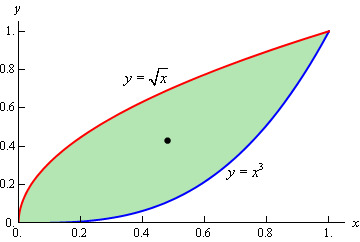
\includegraphics[width=0.5\textwidth]{figures/centreofmassexample}
\end{figure}

\end{frame}

%==============================================================

\begin{frame}[fragile]

\frametitle{$2)$ Applications of integration: \\ \qquad ii) area between curves}

\begin{itemize}
	\item exact area between $f(x) = \sqrt{x}$ and $g(x) = x^3$, domain $[0,1]$ is $5/12 = 0.4166667$
	\item using code \texttt{areabetweencurves.py} for trapezoidal method, $1000$ panels, area is $0.416660$
\end{itemize}

\end{frame}

%==============================================================

\begin{frame}[fragile]

\frametitle{$2)$ Applications of integration: \\ \qquad iii) centre of mass}

Same example as area between curves, but extend to centre of mass at $(\bar{x},\bar{y})$ where

\begin{eqnarray*}
\bar{x} & = & \frac{1}{A} \int_a^b x\left( f(x) - g(x)\right) dx \\
\bar{y} & = & \frac{1}{A} \int_a^b \frac{1}{2} \left( [f(x)]^2 - [g(x)]^2\right) dx
\end{eqnarray*}
where
\[
A = \int_a^b f(x) - g(x) dx
\]

\end{frame}

%==============================================================

\begin{frame}[fragile]

\frametitle{}

\begin{itemize}
	\item Python code: \texttt{centreofmass.py}
\end{itemize}

\begin{figure}[ht]
	\centering
	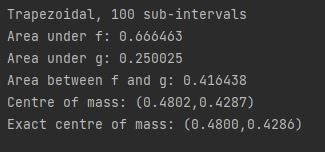
\includegraphics[width=0.5\textwidth]{figures/centreofmassoutput}
\end{figure}
\begin{figure}[ht]
	\centering
	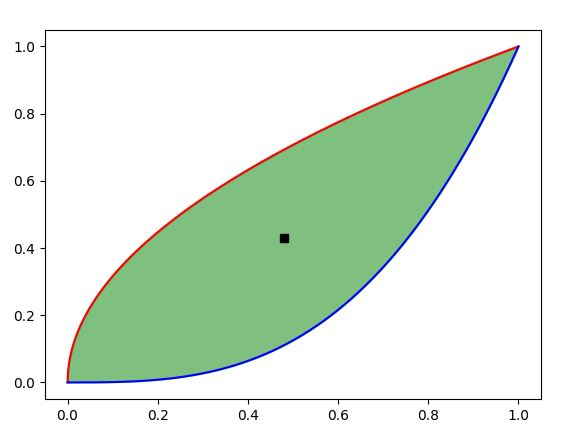
\includegraphics[width=0.5\textwidth]{figures/centreofmassgraph}
\end{figure}

\end{frame}

%==============================================================

\begin{frame}[fragile]

\frametitle{$2)$ Applications of integration: \\ \qquad iv) probability}

probability density function of normal (or Gaussian) distribution:

\[
f(x) = \frac{1}{\sigma\sqrt{2\pi}} e^{-\frac{1}{2}\left(\frac{x-\mu}{\sigma}\right)^2}
\]

\href{https://onlinestatbook.com/2/calculators/normal_dist.html}{https://onlinestatbook.com/2/calculators/normal\_dist.html}

\begin{itemize}
	\item Python code \texttt{normalprob.py}
\end{itemize}

\end{frame}

%==============================================================

\begin{frame}[fragile]

\frametitle{}

\begin{itemize}
	\item normal pdf distribution calculator
\end{itemize}

\begin{figure}[ht]
	\centering
	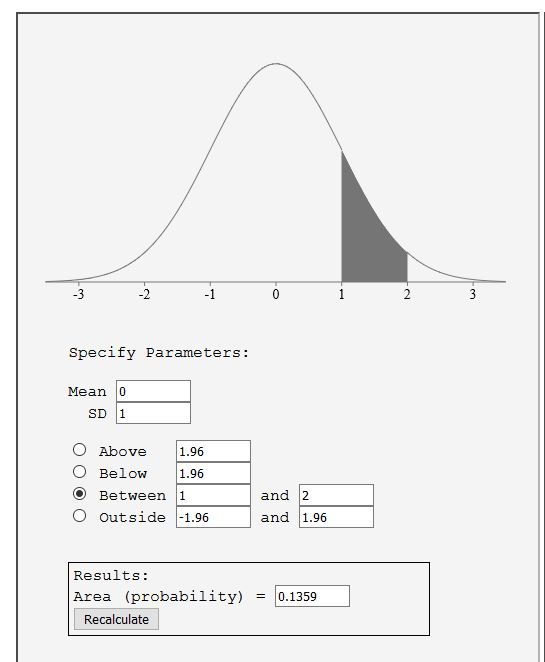
\includegraphics[width=0.5\textwidth]{figures/normalprobcalculator}
\end{figure}

\end{frame}

%==============================================================

\begin{frame}[fragile]

\frametitle{Generate normally distributed random numbers in Python}

\begin{itemize}
%	\item do this???
	\item Python code \texttt{generatenormal.py}
\end{itemize}

\begin{figure}[ht]
	\centering
	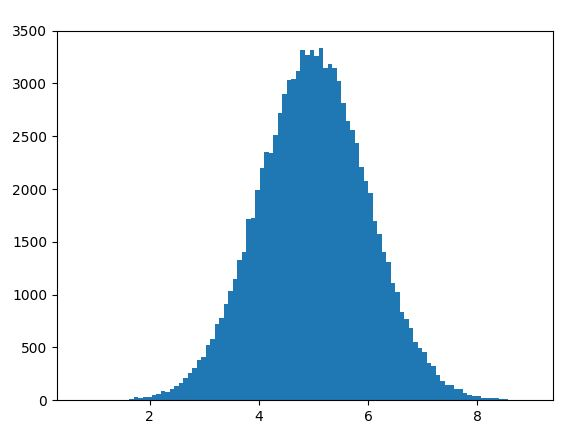
\includegraphics[width=0.5\textwidth]{figures/normalhist}
\end{figure}

\end{frame}

%==============================================================

\begin{frame}[fragile]

\frametitle{$3)$ Interpolation revisited}

\begin{itemize}
	\item xxx
\end{itemize}

\end{frame}

%==============================================================

\begin{frame}[fragile]

\frametitle{Lecture summary}
\begin{itemize}
	\item blah
	\item[]
	
	\item blah

	\item[]
	
	\item blah	
\end{itemize}

\end{frame}


\end{document}